\documentclass{article}
\usepackage{amsmath}
\usepackage{amsthm}
\usepackage{amsfonts}
\usepackage{amssymb}
\usepackage{bbold}
\usepackage{dsfont}
\usepackage{graphicx}
\usepackage{cleveref}
\usepackage{bm}
\usepackage{booktabs}
\usepackage{siunitx}
\usepackage{xcolor}
\usepackage{pdfpages}
\usepackage[utf8]{inputenc}
\usepackage[english]{babel}
\newtheorem{definition}{Definition}
\newtheorem{example}{Example}
\newcommand{\exP}[1]{\mathrm{e}^{#1}}
\newcommand{\dif}{\mathrm{d}}
\renewcommand{\vec}[1]{\mathbf{#1}}
\newcommand{\pdagger}{{\phantom{\dagger}}}
\newcommand{\state}[1]{\vert #1\rangle}
\newcommand{\cstate}[1]{\langle #1\vert}
\newcommand{\outerp}[2]{\vert #1\rangle\!\langle #2 \vert}
\newcommand{\tr}[1]{\mathrm{tr}\left\{#1\right\}}
\newcommand{\trs}[2]{\, \mathrm{tr}_{#1}\{#2\}}
\newcommand{\expc}[3]{\langle #1\vert #2 \vert #3\rangle}
\usepackage[doi=false,url=false,isbn=false,backend=bibtex,style=nature,natbib=true,sorting=none]{biblatex}
\bibliography{bib.bib}
\usepackage{geometry}
\geometry{
	a4paper,
	total={170mm,257mm},
	left=15mm,
	right=15mm,
	top=15mm,
}
\usepackage{kbordermatrix}
\begin{document}
\title{Test of implementation of Subotniks model in the TT formalism}
\author{Rudolf}
\maketitle
\section{Subotniks model}
Two electronic orbitals, $\{1,2\}\otimes \{\uparrow,\downarrow\}$, coupled to two nuclear modes, $x$ and $y$, and two leads \cite{teh2022spin,teh2021antisymmetric}:
\begin{align}
	H &= \frac{P^2}{2M} + H_s + H_b + H_c\\
	H_s &= \sum_{pq} h_{pq}^s(\vec{R}) b_q^\dagger b_p^\pdagger + U(\vec{R})\\
	H_b &= \sum_{k,\alpha=\{L,R\}} \varepsilon_{k\alpha}^\pdagger c_{k\alpha}^\dagger c_{k\alpha}^\pdagger\\
	H_c&= \sum_{p,k\alpha}V_{p,k\alpha}b_p^\dagger c_{k\alpha}+\mathrm{h.c.}\\
	h^{s\uparrow}&=\begin{pmatrix}
		\alpha x+\Delta & Ax-iBy\\
		Ax+iBy & -\alpha x-\Delta
	\end{pmatrix}\\
	h^{s\downarrow} &= (h^{s\uparrow})^*\\
	h_\mathrm{soc} &= \begin{pmatrix}
		0 & \mathrm{A}\\
		\mathrm{A}^\dagger & 0
	\end{pmatrix} \\
	\mathrm{A} &= \frac{\xi \hbar}{2}\begin{pmatrix}
		L_{12}^z & L^-_{12}\\
		L_{12}^+ & -L^z_{12}
	\end{pmatrix}\\
	L^\pm &= L_x \pm i L_y\\
	U(\vec{R})&= \frac{1}{2}x^2 + \kappa_x x + \frac{1}{2}\chi y^2 + \kappa_y y
\end{align}
\clearpage
\section{Isolated Subotnik model: Comparison between TT formalism and exact results}
\begin{figure}[!h]
	\centering
	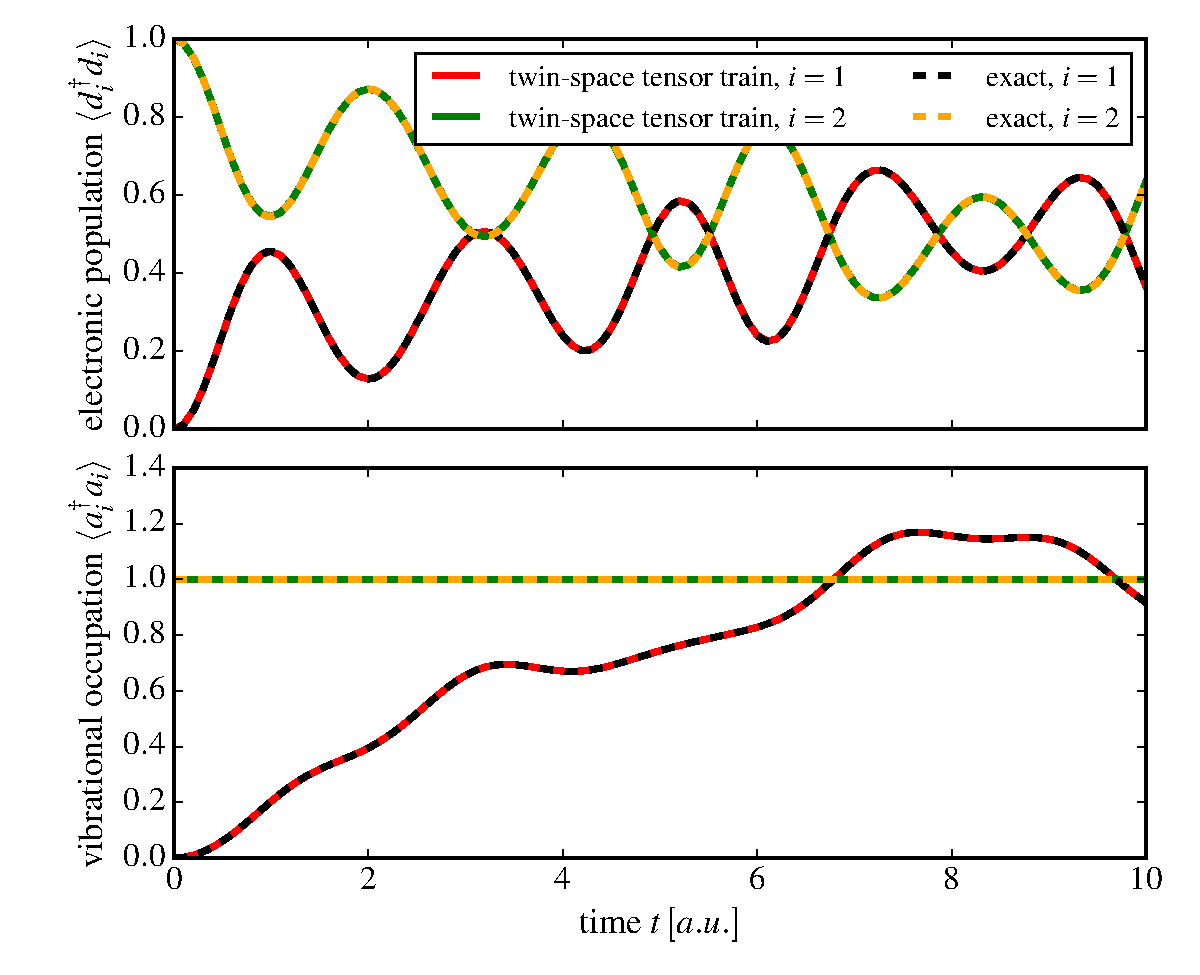
\includegraphics[width=0.9\textwidth]{figs/Comparison_Subotnik_no_spin_Delta_1.0_alpha_0.0_Asoc_0.5_Bsoc_0.0_kappa_0.0_chi_1.0.pdf}
	\caption{$\Delta=1$, $\alpha=0$, $A=1$, $B=0$, $\kappa_x=\kappa_y=0$, $\Omega=1$.}
\end{figure}
\begin{figure}[!h]
	\centering
	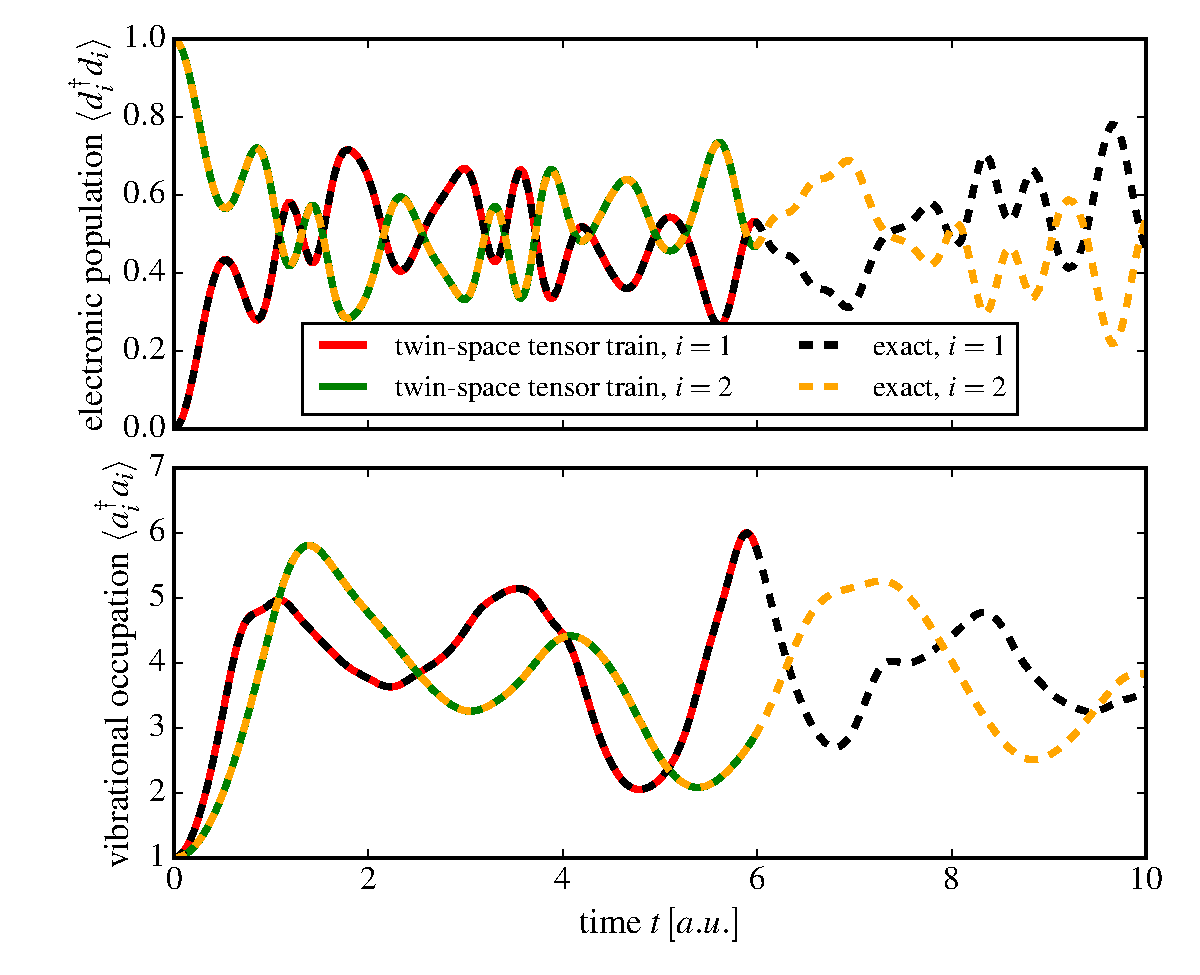
\includegraphics[width=0.9\textwidth]{figs/Comparison_Subotnik_no_spin_Delta_1.0_alpha_1.0_Asoc_-1.0_Bsoc_0.0_kappa_2.0_chi_1.0.pdf}
	\caption{$\Delta=1$, $\alpha=1$, $A=1$, $B=0$, $\kappa_x=\kappa_y=2$, $\Omega=1$.}
\end{figure}
\begin{figure}[!h]
	\centering
	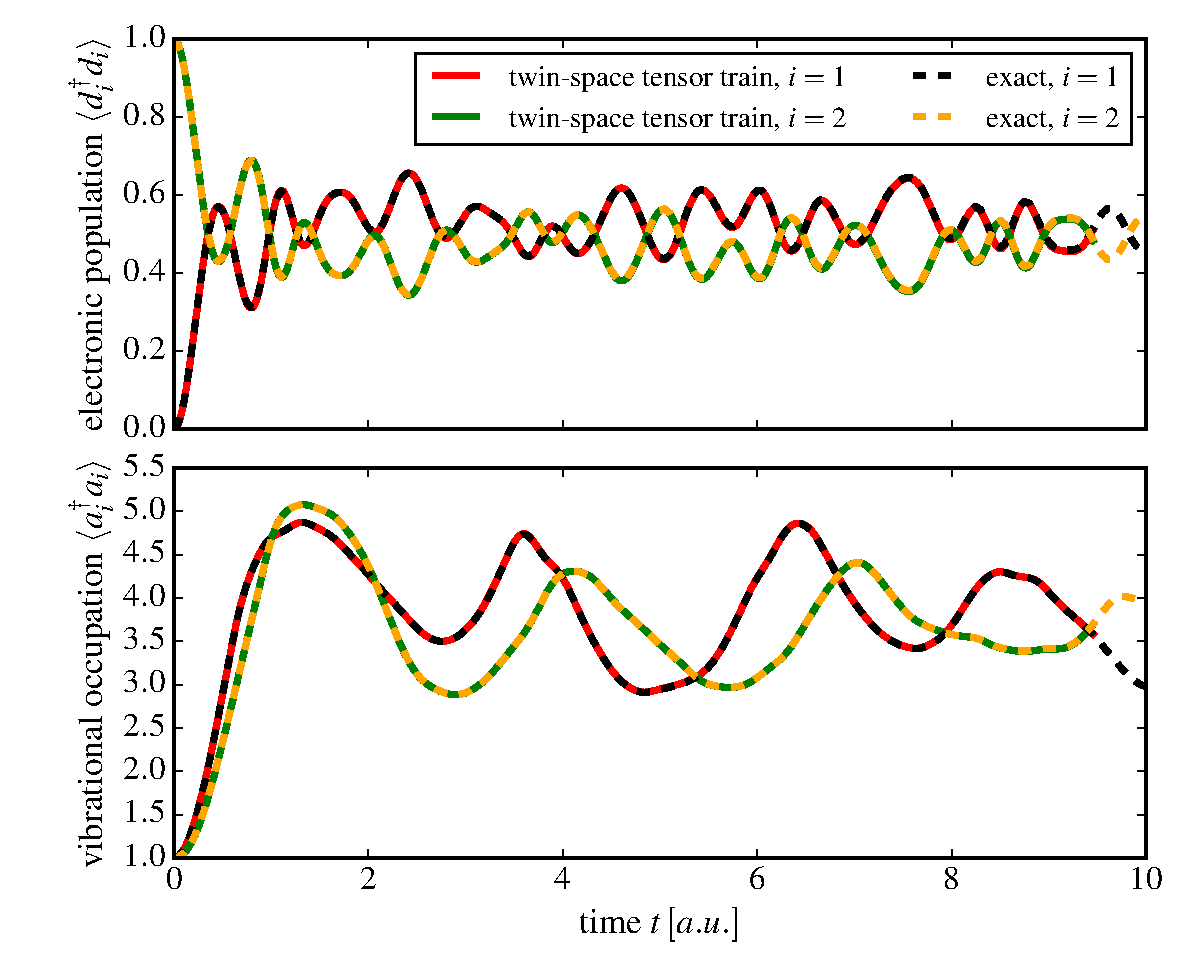
\includegraphics[width=0.9\textwidth]{figs/Comparison_Subotnik_no_spin_Delta_1.0_alpha_1.0_Asoc_-1.0_Bsoc_-1.0_kappa_2.0_chi_1.0.pdf}
	\caption{$\Delta=1$, $\alpha=1$, $A=1$, $B=1$, $\kappa_x=\kappa_y=2$, $\Omega=1$.}
\end{figure}
\clearpage

\printbibliography
\end{document}


